\chapter{Methodology}
\label{chap:ch4}

In this chapter I will describe the implementation of the three main steps taken by the engine to find the best move: generating legal moves for a position, searching for legally reachable positions from the current position, and then evaluating each one and determining which one is the best \cite{marsland1986review}.

% Description of the approach taken to build the chess engine
% Explanation of the AI techniques used and why they were chosen

\section{Move generation}
\label{sec:ch4sec1}

The engine computes the pseudo-legal moves of the pieces of the player that is moving, then it does each move, checks the state of the board, adds the move to the list of legal moves if the board is in a valid state, and then undoes the move.

To check the state of the board I used a threat map (fig. \ref{fig:threatMap}), which keeps track of the squares that are under attack or are defended by at least one piece (including empty squares, squares with allied pieces, and squares with opponent pieces). After each move, the threat map is updated in the following way: for each white piece on the board, it sets "IsAttackedByWhite" to true for all the squares it attacks, and for each black piece on the board, it sets "IsAttackedByBlack" to true for all the squares it attacks.

\begin{figure}
  \centering
  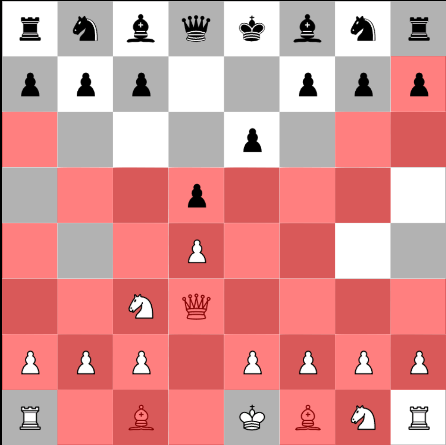
\includegraphics[scale=0.5]{figures/white-threat-map.png}
  \captionof{figure}{White threat map}
  \label{fig:threatMap}
\end{figure}

\section{Search}
\label{sec:ch4sec2}

The simplest way of searching in the game tree is through a fixed depth Minimax algorithm, which would be mathematically accurate, but would not yield good results and would be very slow. However, in combination with some optimizations and heuristics, it can compute faster and find better moves.

\subsection{Alpha-beta pruning}
\label{subsec:ch4sec2subsec1}

The Minimax algorithm was improved with Alpha-beta pruning, which preserves the accuracy of the algorithm and significantly reduces the number of nodes visited if combined with a good move ordering heuristic \cite{eric1992analysis}.

A simple pseudocode for Alpha-beta pruning is shown in fig. \ref{fig:alphabetaPseudocode}:

\begin{figure}[h]
  \centering
  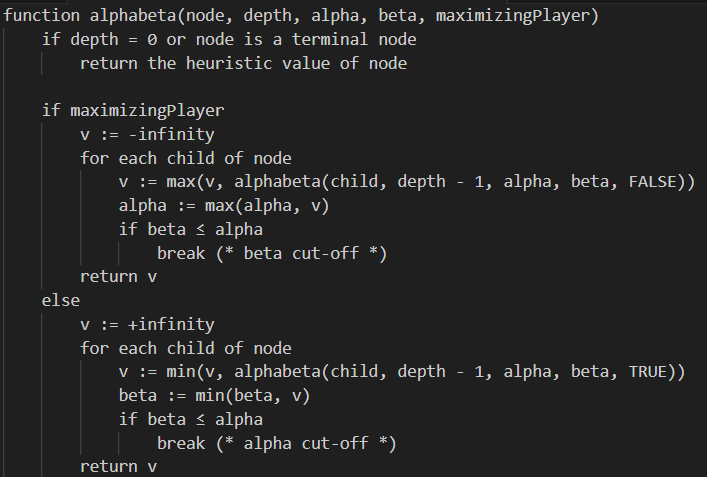
\includegraphics[scale=0.9]{figures/alphabeta-pseudocode.png}
  \captionof{figure}{Alpha-beta pruning pseudocode}
  \label{fig:alphabetaPseudocode}
\end{figure}

The heuristic I used in combination with Alpha-beta pruning is MVV-LVA (Most Valuable Victim - Least Valuable Agressor): the moves that capture pieces with high values are first, and if multiple moves capture a piece of the same value, the moves with the least valuable agressor are prioritized \cite{mvv-lva}. The heuristic is based on the observation that in chess, it is often advantageous to capture pieces of higher value than the capturing piece, while avoiding exchanges where the capturing piece is more valuable than the captured piece. It is also relatively easy to implement, and does not require much computational overhead. Other heuristics, use the evaluations of previous searches or the results from other branches, and require maintaining and updating additional data structures to keep track of the move history and their performance.

\subsection{Quiescence search}
\label{subsec:ch4sec2subsec2}

When the Minimax search reaches the maximum depth in a branch, it evaluates the position and propagates it back. With the quiescence search optimization, the position is first checked for potential moves that could disrupt the evaluation in the following move.

I considered captures and promotions to be disruptive moves, since they have a big impact on material. If there are no such moves available, the algorithm continues as normal. But if there are, the current static evaluation is kept as a "stand-pat" score (the term is used in poker, to describe a situation where a player chooses to keep their hand as it is without drawing any additional cards), to establish a lower bound on the evaluation.

The "disruptive" moves are played, and, from the positions reached, quiescence search is applied again, until a certain depth is reached. Each new position is evaluated using the static function, and if the evaluation is better than alpha (the lower bound, which is initialized with the stand-pat score), then the evaluation score is assigned to alpha. At the end of the quiescence search, the alpha score is returned. I used 4 as the maximum quiescence search depth, to allow the engine to detect certain series of exchanges, but not search too deep and use up too much time.

The stand-pat score is used based on the Null Move Observation, which states
that there is almost always a move that improves the current position - it assumes the player to move is not in Zugzwang (a position in which it is disadvantageous to move, as every move inevitably results in a worse position). The stand-pat assumes that even if all the disruptive moves are searched, and none of them increase alpha, one of the non-disruptive moves can most likely raise alpha. This is not valid if every move is searched.

\subsection{Iterative deepening}
\label{subsec:ch4sec2subsec3}

The iterative deepening starts computing the evaluations for the Minimax with depth 1, and then increments the depth up to the given maximum depth. After the time given as an input elapses, the search is stopped and the move with the best evaluation found on the previous depth search is returned. I set the maximum time to 50 seconds, but this can be easily changed from a parameter, depending on the length of the match and accuracy of moves the user of the engine desires.

\section{Evaluation}
\label{sec:ch4sec3}

I used two methods of evaluating a chess board position. The first one is a simple evaluation function based on the position of the pieces on the board, and the second one is a neural network model, trained on matches played at grandmaster level.

\subsection{Board pieces}
\label{subsec:ch4sec3subsec1}

This evaluation function assigns a value to the board configuration based on the position of the pieces and the state of the game (opening/middlegame/endgame). I considered the state to be the opening if there were less than 13 moves made, middlegame if there are at least a queen or 3 minor pieces (rook/bishop/knight) on the board, and the endgame otherwise.

\begin{figure}[h]
    \centering
    \begin{minipage}{.49\textwidth}
      \centering
      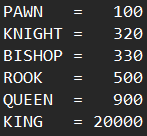
\includegraphics{figures/pieces_values.png}
      \captionof{figure}{Base values for the pieces}
      \label{fig:piecesValues}
    \end{minipage}
    \begin{minipage}{.49\textwidth}
      \centering
      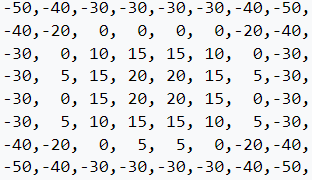
\includegraphics{figures/knight_value_table.png}
      \captionof{figure}{Knight value table}
      \label{fig:knightValueTable}
    \end{minipage}
\end{figure}

\begin{figure}[h]
    \centering
    \caption{King value tables}
    \begin{subfigure}{0.49\textwidth}
        \centering
        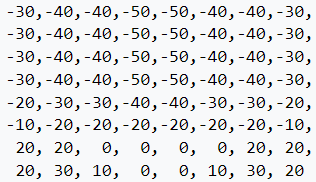
\includegraphics{figures/king_value_table_middlegame.png}
        \caption{King middlegame value table}
        \label{fig:kingValueTableMiddlegame}
    \end{subfigure}
    \begin{subfigure}{0.49\textwidth}
        \centering
        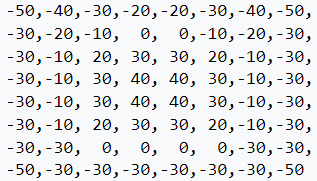
\includegraphics{figures/king_value_table_endgame.png}
        \caption{King endgame value table}
        \label{fig:kingValueTableEndgame}
    \end{subfigure}
\end{figure}

Each piece has a base value (fig. \ref{fig:piecesValues}), to which another value is added based on the square the piece occupies. Each piece has an 8x8 table, with a value for each square. The tables contain values as to encourage development of the pieces (example - fig. \ref{fig:knightValueTable} shows the table for the white knights). The tables for black pieces are horizontally simetric to the ones for the white pieces. The king has an additional table for the endgame, because in the opening and middlegame it is encouraged to castle and discouraged to move far from the first rank (fig. \ref{fig:kingValueTableMiddlegame}), while in the endgame it is encouraged to go towards the center and play an active part in the game (fig. \ref{fig:kingValueTableEndgame}) \cite{wikiEval}.

\subsection{Neural network}
\label{subsec:ch4sec3subsec2}

For the second evaluation function, I trained a neural network on grandmaster chess matches.

\subsubsection{Dataset}
\label{subsec:ch4sec3subsec2subsubsec1}

The dataset consists of chess matches played at grandmaster level downloaded in PGN format from the website chessabc.com \cite{chessabc}.

A PGN (portable game notation) file contains multiple chess matches. Each match has several headers (name of player with white pieces, name of player with black pieces, event it was played at, date it was played on, result, elo of players etc.), an empty line, and then the "movetext section". The matches in a PGN file are separated by two empty lines. Following is a sample PGN match:
\begin{figure}[h]
    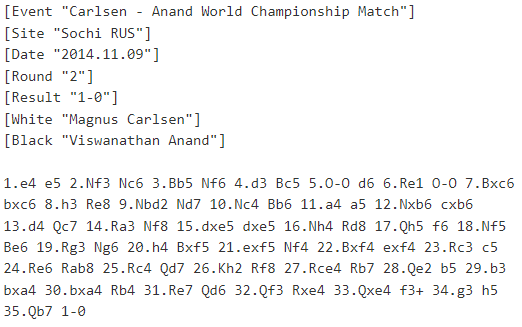
\includegraphics[width=0.8\textwidth]{figures/carlsen-anand-match.png}
\end{figure}

The movetext section contains the chess moves, move numbers, optional annotations and a concluding game termination marker (the result of the match). The result can be "1-0" (white won), "0-1" (black won) or "1/2-1/2" (draw). The moves are written in SAN (standard algebraic notation). SAN identifies each square on the board as a combination of file (a-h) and rank (1-8) (see fig. \ref{fig:boardSquares}).

\begin{figure}[h]
    \centering
    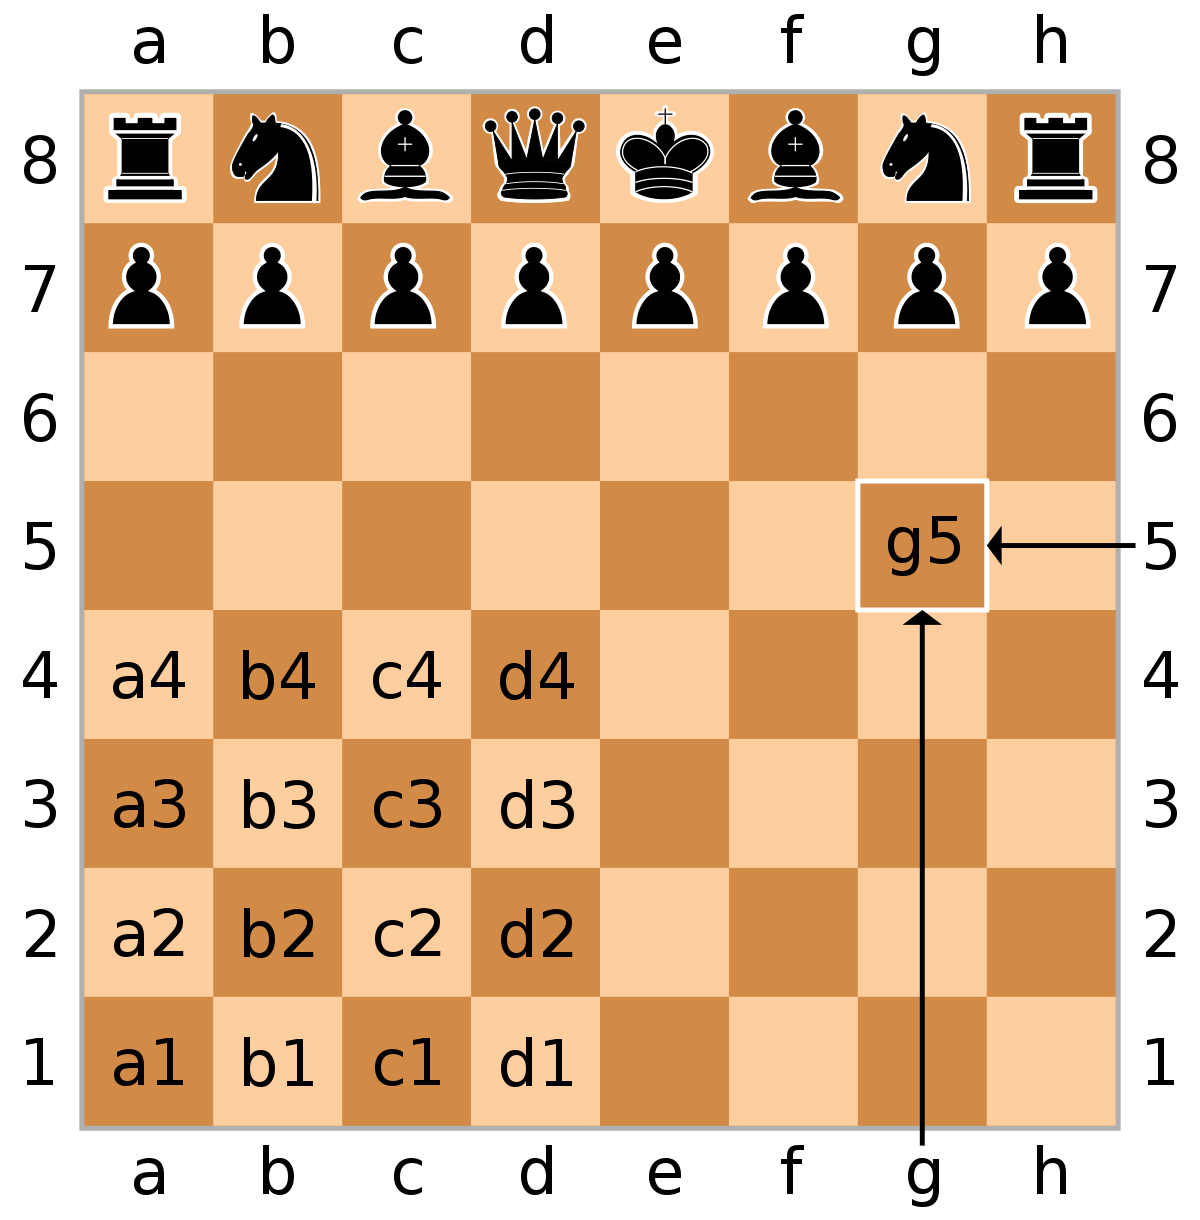
\includegraphics[width=0.4\textwidth]{figures/board-squares.png}
    \caption{Board squares}
    \label{fig:boardSquares}
\end{figure}

Each piece can be identified by a letter (K - king, Q - queen, R - rook, B - bishop, N - knight, P - pawn). Simple SAN moves contain only the destination square, and the letter of piece that moves, if the piece is not a pawn (for example, pawn to c6 is written simply as c6, while knight to c6 is written as Nc6). There are additional rules for moves \cite{edwards1994standard}:
\begin{itemize}
    \item Moves that capture a piece contain the 'x' character right before the destination square (ex: Bxb4)
    \item Castling kingside is written as 'O-O', while queenside castling is written as 'O-O-O'
    \item Moves of pawns to the last rank (promotion moves) contain the equal sign ('=') right after the destination square, followed by the letter of the piece that the pawn promotes to (ex: e8=Q)
    \item If there are multiple pieces of the same type that can move to the destination square, the file of the originating square is added right after the piece (ex: Nbc6); if this does not solve the ambiguation, the rank of the originating square is added instead (ex: N8c6), and if neither of these works, both the file and the rank are added (ex: Nb8c6)
    \item If the move checks the opponent's king, a plus sign ('+') is added at the end of the move (ex: Qe7+); if the move checkmates the opponent's king, the octothorpe sign ('\#') is added instead (ex: Qe7\#)
\end{itemize}

I computed the positions that occured in the matches in the dataset, and the value I assigned to each position is the mean of the results of the matches in which the position appeared. For example: if a certain position appeared in 10 matches, and 4 of the matches ended in a win for white, 2 in a win for black, and the other 4 were draws, the value assigned to the position is: \[\frac{(4*1)+(2*-1)+(4*0)}{10}=0.2\] (a win for white is assigned 1, a win for black is assigned -1, and a draw is 0).

% Number of positions: 8493798, number of distinct positions: 5586478

There are a number of 8.5 million positions in the dataset, and 5.5 million of those positions are distinct.

\subsubsection{Model}
\label{subsec:ch4sec3subsec2subsubsec2}

The model receives as input a position and outputs a value between -1 (winning for black) and 1 (winning for white). The position is encoded as 70 values. Following is the encoding for the starting position:

$4,1,0,0,0,0,7,10,2,1,0,0,0,0,7,8,3,1,0,0,0,0,7,9,5,1,0,0,0,0,7,11,6,1,0,$

$0,0,0,7,12,3,1,0,0,0,0,7,9,2,1,0,0,0,0,7,8,4,1,0,0,0,0,7,10,1,1,1,1,-1,0$

The input layer contains 70 nodes. The first 64 values describe the positions of the pieces (first 8 values are the pieces on a1, a2, a3, ..., a8, then b1, b2, b3, ..., b8, etc.) - each square is assigned a value based on the piece it contains (see fig. \ref{fig:squaresEncodedValues}). The next 4 values are boolean (0 - false, 1 - true) and encode the castling rights (white can castle kingside, white can castle queenside, black can castle kingside, and black can castle queenside). The next value is the en passant file (the file of the moved pawn, encoded from 0 to 7, if the last move pushed a pawn two squares, -1 otherwise). The last value is the player to move (0 for white, 1 for black).

\begin{figure}[h]
    \centering
    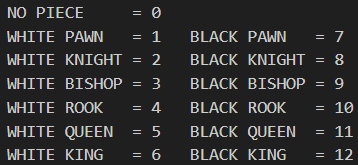
\includegraphics[width=0.6\textwidth]{figures/squares-encoded-values.png}
    \caption{Squares encoded values}
    \label{fig:squaresEncodedValues}
\end{figure}

There is only one hidden layer, with 32 nodes, with a Rectified Linear Unit (ReLU) activation function.

The output layer contains one node, the evaluation of the position, with a hyperbolic tangent (Tanh) activation function, so the output is between -1 and 1.

\subsubsection{Training}
\label{subsec:ch4sec3subsec2subsubsec3}

% 100 epoci, batch-size 64

The model was trained for 100 epochs, on a batch-size of 64, using Stochastic Gradient Descent (SGD) as an optimizer and Mean Squared Error (MSE) as a loss function.